\documentclass{beamer}

\usepackage{geometry}
\usepackage{graphicx}
%\usepackage{wrapfig}
\usepackage{amsmath}

%\useoutertheme{infolines}
\usetheme{Boadilla}
\usecolortheme{seahorse}
\setbeamertemplate{navigation symbols}{}
\title{Memory Mapping in 64 Bit Mode}
\newcommand{\shorttitle}{64 Bit Intel Assembly Language}
\newcommand{\shortauthor}{\copyright 2011 Ray Seyfarth}
\author{Ray Seyfarth}
\begin{document}


\usefoottemplate{\vbox{
\tinycolouredline{structure!55}%
 {\color{white}{\textbf{\shorttitle}\hfill\textbf{\shortauthor}}}%
}}

\begin{frame}
    \titlepage
\end{frame}
\begin{frame}
\frametitle{Outline}
\tableofcontents
\end{frame}

\section{Memory mapping basics}


\begin{frame}
    \frametitle{Memory mapping register}
    \begin{itemize}
        \item Named ``Control Register 3'' or {\tt CR3}
        \item Contains the physical address of the top-level of the memory
              mapping tables
        \item There are 4 levels in a hierarchy of tables for memory mapping
        \item Memory mapping tables are setup and then CR3 is set to the
              address of top table.
        \item The top table is called ``Page Map Level 4'' or {\tt PML4}
    \end{itemize}
\end{frame}

\begin{frame}
    \frametitle{Memory mapping pages and tables}
    \begin{itemize}
        \item Each page is $2^{12} = 4096$ bytes
        \item An address is 8 bytes
        \item Each page can hold $2^9 = 512$ addresses
        \item A 9 bit field is needed to index the mapping tables
        \item In general if pages are size $2^k$, then a page can hold $k-3$ pointers
        \begin{itemize}
            \item I think $2^{15}=32768$ would be nice for a page size
            \item We could use 12 bits for page table indices 
            \item 3 levels for 36 bits would be enough page hierarchy levels
            \item Total memory limit would $2^{51} = 2,251,799,813,685,248$
            \item 2 Petabytes of RAM might be enough for most personal computers
        \end{itemize}
        \item Current mapping uses $48$ bits, we we are limited to $2^{48}$ bytes which is about 262 Terabytes
    \end{itemize}
\end{frame}

\begin{frame}
    \frametitle{Logical memory address fields}
    \begin{center}
        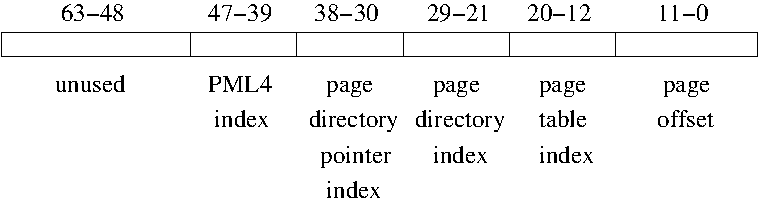
\includegraphics[width=0.95\textwidth]{address.pdf}
    \end{center}
    \begin{itemize}
        \item Bits 47-39 are used to index the PML4 table
        \item Bits 38-30 are used to index the selected page directory pointer table
        \item Bits 29-21 are used to index the selected page directory table
        \item Bits 20-12 are used to index the selected page table
        \item Bits 11-0 are the offset into the page (for 4 KB pages)
    \end{itemize}
\end{frame}

\section{Page map level 4}
\begin{frame}
    \frametitle{Page map level 4}
    \begin{itemize}
        \item Assume {\tt CR3} has the physical address {\tt 0x4ffff000}
    \end{itemize}
    \begin{center}
        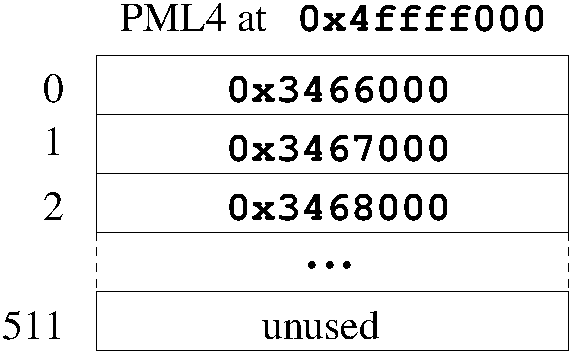
\includegraphics[width=0.40\textwidth]{pml4.pdf}
    \end{center}
    \begin{itemize}
        \item Let's translate logical address {\tt 0x80801fffa8}
        \item Bits 47-39 = 1, so we use the second entry
        \item The page directory pointer table we need is at {\tt 0x3467000}
    \end{itemize}
\end{frame}

\section{Page directory pointer table}

\begin{frame}
    \frametitle{Page directory pointer table}
    \begin{center}
        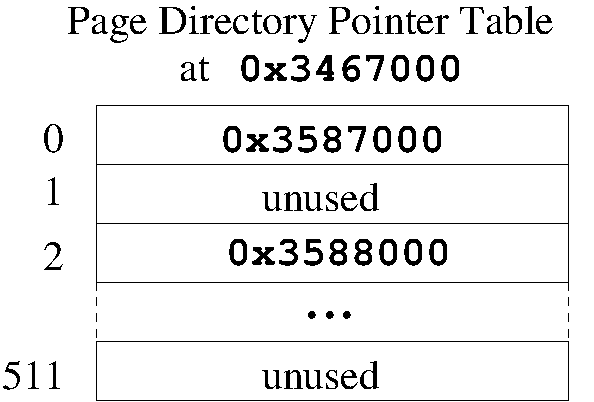
\includegraphics[width=0.40\textwidth]{pdptable.pdf}
    \end{center}
    \begin{itemize}
        \item We're translating logical address {\tt 0x80801fffa8}
        \item Bits 38-30 = 2, so we use the third entry
        \item The page directory table we need is at {\tt 0x3588000}
    \end{itemize}
\end{frame}

\section{Page directory table}

\begin{frame}
    \frametitle{Page directory table}
    \begin{center}
        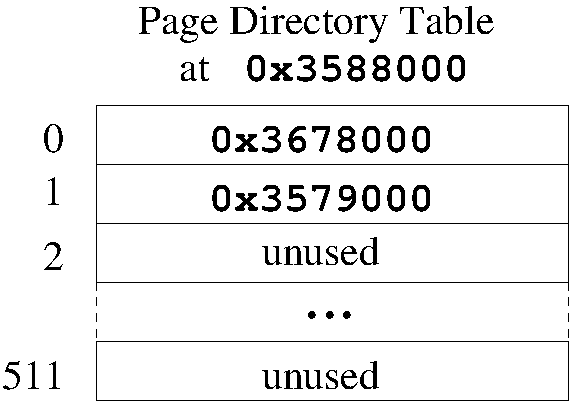
\includegraphics[width=0.40\textwidth]{pdtable.pdf}
    \end{center}
    \begin{itemize}
        \item We're translating logical address {\tt 0x80801fffa8}
        \item Bits 29-21 = 0, so we use the first entry
        \item The page table we need is at {\tt 0x3678000}
    \end{itemize}
\end{frame}

\section{Page table}

\begin{frame}
    \frametitle{Page table}
    \begin{center}
        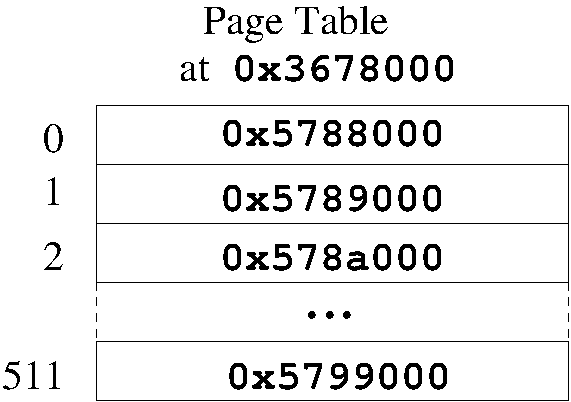
\includegraphics[width=0.40\textwidth]{ptable.pdf}
    \end{center}
    \begin{itemize}
        \item We're translating logical address {\tt 0x80801fffa8}
        \item Bits 20-12 = 511, so we use the last entry
        \item The page we need is at {\tt 0x5799000}
        \item So logical address {\tt 0x80801fffa8} is at physical
              address {\tt 0x5799fa8}
    \end{itemize}
\end{frame}

\section{Large pages}

\begin{frame}
    \frametitle{Large pages}
    \begin{itemize}
        \item Using the first 3 existing levels of page tables, we can have
              large pages with $2^{21}= 2097152$ bytes
        \item This is used by Linux for the kernel
        \item By allocating some memory for large pages, user programs
              can use large pages
        \item By using 1 byte per page on 8 GB of data, I managed to have
              more need for cache for page table entries than my computer had
        \item Performance was significantly slower
        \item Large database memory regions would benefit greatly from
              using 2 MB pages
    \end{itemize}
\end{frame}

\section{CPU support for fast lookups}

\begin{frame}
    \frametitle{CPU support for fast lookups}
    \begin{itemize}
        \item A CPU uses a special cache called a ``Translation Lookaside Buffer'' or TLB to speed up memory translation
        \item A TLB operates much like a hash table
        \item Presented with a logical address, it produces the physical address
              or failure in about $1/2$ a clock cycle
        \item The Intel Core i7 has 2 levels of TLBs
        \begin{itemize}
            \item Level 1 holds 64 small page translations (or 32 big pages)
            \item Level 2 holds 512 page translations
            \item Large programs with small pages will experience TLB misses
                  which can be satisfied fairly rapidly with normal cache
            \item Very large programs can crawl
        \end{itemize}
    \end{itemize}
\end{frame}

\end{document}
